\chapter{Background \& Related Work}\label{ch:background}

\section{General Challenges of Computer Vision}

\subsection{The Semantic Gap}

One of the core insights of computer vision in general and content based image
retrieval in particular probably is that human perception is inseparably linked
to interpretation by the brain. As a human individual there is no way to
directly access visual information without them having been filtered and
weighted by one's personal experiences and cultural context. Therefore, when
people talk about visual similarity of images, it usually includes a large
degree of semantic similarity unconciously added to the perception. The
difference between that mode of perception and the current algorithmic ways to
analyse visual data has been eloquently coined \emph{the semantic gap} by
Smeulders et al.\ \autocite{smeulders_content-based_2000}:

\begin{quote}
"The semantic gap is the lack of coincidence between the information that one
can extract from the visual data and the interpretation that the same data have
for a user in a given situation."
\end{quote}

Having had that realisation can guide the decision of a researcher or designer
of such systems.

\subsection{The Sensory Gap}

In addition to the semantic ambiguity described above, another major obstacle
of computer vision impacts a CBIR system: \emph{the sensory gap}. This term has
also been coined by Smeulders et al.\ \autocite{smeulders_content-based_2000},
who define it as follows:

\begin{quote}
"The sensory gap is the gap between the object in the world and the information
in a (computational) description derived from a recording of that scene."
\end{quote}

That terse definition includes a multitude of conditions, that can affect an
image, which a CBIR system operates on:

\begin{description}
    \item[Illumination] The brightness or direction of the illumination can
        hide or accent edges and texture properties in the scene. Similarly,
        the color of the illumination influences the recorded color information
        in the image.
    \item[Resolution] The imaging resolution sets a lower limit on the size of
        features that can be correctly recognised by any algorithm. As in all
        signal processing applications, aliasing of high frequency components
        of the image can introduce further ambiguities.
        \autocite{shannon_communication_1998}
    \item[Occlusion] Depending on the viewpoint of the recording and the
        composition of the scene, distinguishing parts of depicted objects may
        be occluded by other objects or objects may be only partially inside
        the recorded image.
    \item[Perspective] An object's proportions can be distorted by the imaging
        perspective.
\end{description}

An ideal CBIR system would use feature extraction and comparison methods that
can account and correct for such conditions.

\section{Anatomy of a CBIR System}\label{sec:anatomy}

The inner workings of most CBIR systems can best be examined by looking at the
processing pipeline each query has to go through. The coarse sequence of
computational steps is almost the same in all such systems (Figure
\ref{fig:cbir_coarse_structure}):

\begin{enumerate}
    \item Acquire the image.
    \item Extract the signature using a feature extraction algorithm.
    \item Compare the signature to a database containing the signatures of the
        images to search within.
    \item Rank the images by similarity using the comparison results.
\end{enumerate}

\begin{figure}[h]
    \centering
    \subfloat[Local features]{%
        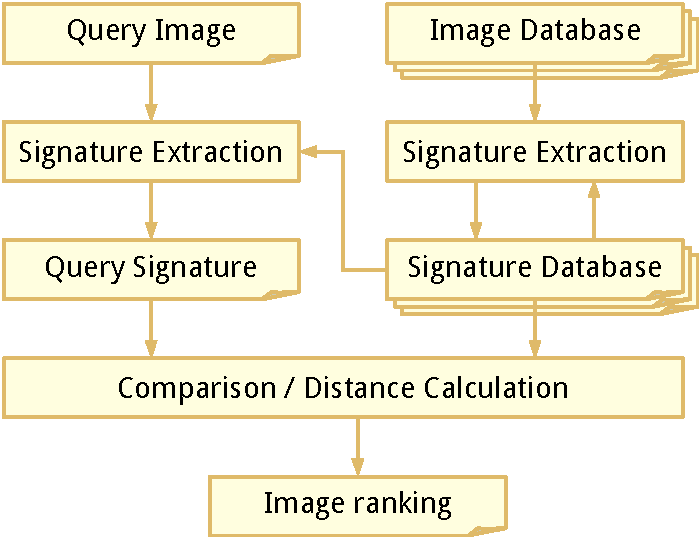
\includegraphics[width=0.45\textwidth]{cbir_anatomy_query_local_cropped}%
        \label{fig:cbir_coarse_structure_local}%
    }
    \quad
    \subfloat[Global features]{%
        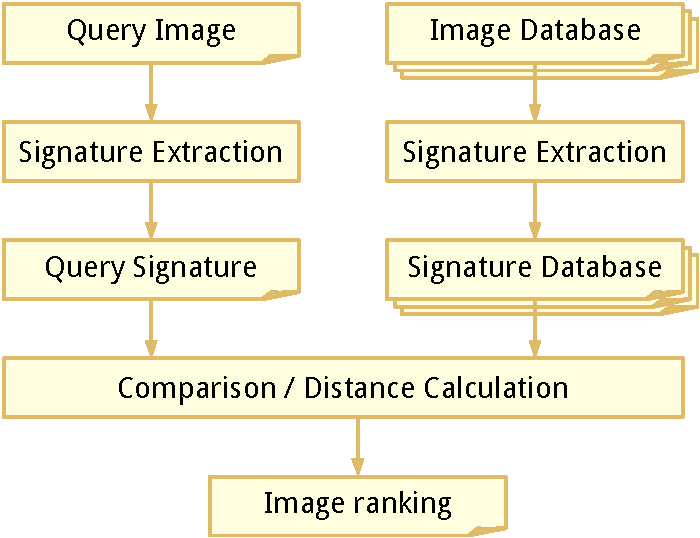
\includegraphics[width=0.45\textwidth]{cbir_anatomy_query_cropped}%
        \label{fig:cbir_coarse_structure_global}%
    }
    \caption[Coarse structure of a CBIR system]{
        The processing pipeline for CBIR using both local and global features
        is very similar. The main difference is in the signature extraction
        step, in which local features are selected, weighted and/or compressed
        depending on the results of the signature extraction of the other
        images in the database.
    }
    \label{fig:cbir_coarse_structure}
\end{figure}

\subsection{Image Acquisition}\label{sec:anatomy_image_acquisition}

The format in which the images are available to the system determines the
maximum amount of information available to subsequent analysis steps.

A significant part of the preprocessing usually done after acquisition depends
on the broadness of the image domain. The concept of the domain encompasses and
describes the variability of many possible image parameters like illumination
or composition and is therefore closely related to the sensory gap described
above. The narrower the image domain is, the more assumptions the system can
make about image from that domain. By their very nature, the domain of sketch
based image retrieval systems is usually very broad. It contains the sketches
create by the user to query the database as well as the images in the database
itself, which can be of a completely different nature, e.g.\ photos or
paintings.

Another factor usually is the accepted input format of the feature extraction
algorithm. Many algorithms like SIFT \autocite{lowe_object_1999} or SURF
\autocite{bay_speeded-up_2008} are defined for single-channel data, but some
have been specifically developed to operate on multi-channel images, like cSIFT
\autocite{abdel-hakim_csift:_2006} and \autocite{yang_robust_2008}.

\subsection{Signature Extraction}\label{sec:anatomy_signature_extraction}

The signature of an image is its representation in the following comparison
step. Therefore it should describe the image using its most discriminatory
features compared to all other images in the database. Due to the effects of
the \emph{sensory gap} discussed above, there is, at the moment, no definitive
way to determine the discriminatory power of features in general, even though
knowledge about the image domain can guide the descisions.  The signature
composition depends on both, the kind of features extracted from the image and
the way these features are encoded. 

Over the last two decades, a wide variety of feature descriptors have been
published, which mostly focus on specific types of features. Some techniques
use color histograms \autocite{utenpattanant_color_2006}, while others
\autocite{stricker_color_1996} \autocite{deng_efficient_2001}
\autocite{lee_spatial_2003} include spatial relations between colors in a
region.
Many descriptors attempt to capture texture characteristics, such as
\autocite{schaffalitzky_viewpoint_2001} and \autocite{manjunath_texture_1996}.
Rubner and Thomasi \autocite{rubner_texture-based_1999} combine Gabor filters
and the earth mover's distance and thereby bypass segmentation.
Another class of descriptors focuses on representing shapes using detection of
edges and salient points. Lowe \autocite{lowe_object_1999} developed the now
widely adopted SIFT descriptor, that employs clustering of salient points. More
recently, the SURF desciptor \autocite{bay_speeded-up_2008} uses Haar wavelets
to deliver comparable performance.
Several publications combine feature types to arrive at a more comprehensive
descriptor. Oliva and Torralba \autocite{oliva_modeling_2001} capture various
scene properties like "roughness" and "openness".

\begin{figure}[h]
    \centering
        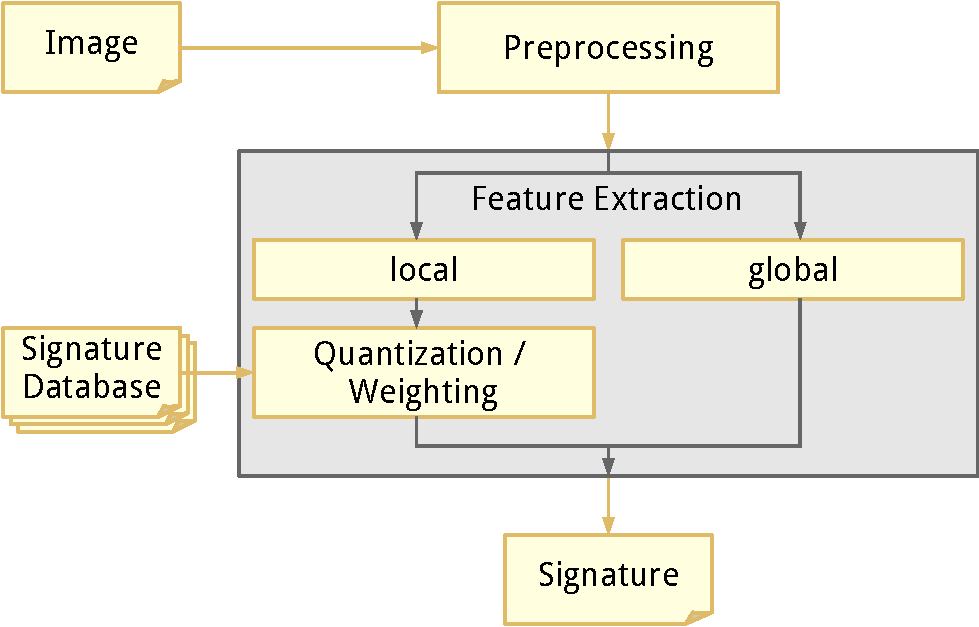
\includegraphics[width=0.8\textwidth]{cbir_anatomy_signature_extraction_cropped}
    \caption{Signature extraction in CBIR systems}
    \label{fig:cbir_signature_extraction}
\end{figure}

\subsubsection{Global Features}

Aside from the nature of the features captured by a descriptor, there are also
differences in the geometrical scope the features are derived from. Global
feature descriptors attempt to capture the structure of the whole scene or
describe the distribution of properties across the image like the binary Haar
color descriptor published in \autocite{utenpattanant_color_2006}. Some global
algorithms subdivide the image into regular segments and derive the localized
distribution of features for each division. \autocite{lazebnik_beyond_2006}
improves upon this concept by creating feature pyramids using iterative
subdivision for multiscale analysis. While the computational complexity of
those global approaches is usually quite low, they are especially susceptible
to problems like partial occlusion or reflections within the scene. The spatial
envelope descriptor \autocite{oliva_modeling_2001} combines a global
spectrogram with locally derived spectral information to produce an overall
image descriptor.

\subsubsection{Local Features}

In contrast to the global approach, many CBIR systems employ "bag-of-features"
descriptors, that represent the image as an unsorted collection of local
features extracted from small patches of the image. The unsorted nature of the
feature collection leads to loss of large-scale geometric structures that can
be counteracted by a suitable choice of the patch sizes. When the local feature
descriptors are invariant to rotation, scale or similar deformations, the
sensitivity to viewpoint variations or occlusions decreases. The prominent SIFT
descriptor \autocite{lowe_object_1999} achieves this by selecting the feature
locations such that they can be normalized with respect to scale, orientation
and limited 3D projections. The SURF descriptor by Bay et al
\autocite{bay_speeded-up_2008} gives similar results, but has reduced
computational requirements. The HOG descriptor \autocite{dalal_histograms_2005}
calculates histograms of gradient directions on regular grid cells to describe
the local angular distribution of edges.

\subsubsection{Dimensionality Reduction}

The signatures produced by local descriptors are often large sets of vector,
that are themselves of considerable size. For example, the SIFT descriptor
describes each image using about $1000$ local feature vectors of $160$ values
each. Such large numbers of vectors are expensive to store and compare, so one
of several data reduction methods is commonly used.

\paragraph{Principal Component Analysis}

The Principle Component Analysis (PCA) is a transformation, that computes the
orthogonal basis best suited to describe the variance of the data. An
$n$-dimensional data set is linearly mapped to a coordinate system, in which
the direction of the first axis $a_1$ is the direction with the largest
variance in the data. The following axes' $a_i$, $i \in 2, \dots, n$ directions
correspond to the orthogonal directions with the next-largest variances in
descending order. By choosing the $p$ largest component vectors and performing
an inverse transformation of the PCA-transformed data, a projection of the
original data in $p$ dimensions can be obtained. Due to the choice of the
vectors for the inverse transformation, the projection discards only the parts
of each observation that vary the least between all observations.

PCA has been applied to the face recognition problem using intensity images
(eigenfaces) \autocite{turk_face_1991}, wavelets (waveletfaces)
\autocite{feng_human_2000} and more recently curvelets (curveletfaces)
\autocite{mandal_face_2008}. In \autocite{ke_pca-sift:_2004} it was used to
improve the robustness of the SIFT \autocite{lowe_object_1999} descriptor. To
overcome the limited between-class discrimination of PCA, it has been combined
with Linear Discriminant Analysis (LDA), yielding even better results
\autocite{mandal_curvelet_2009}.

\paragraph{Visual Words and Clustering}

Instead of reducing the size of the individual feature vectors, the
bag-of-features approach collects the feature vectors into a single signature
vector to represent the image. This is done by determining a codebook of
representative feature vectors, the "visual words" \autocite{sivic_video_2003},
and assigning each local feature vector to the most similar visual word. A
histogram of the distribution of visual words can then be calculated as a
signature for each image.

To create the codebook, the large number of feature vectors extracted from
local patches of each image in the database are grouped into clusters of
similar vectors. The optimal number of clusters is usually determined
experimentally and varies with other processing parameters such as the sampling
strategy \autocite{nowak_sampling_2006} \autocite{yang_evaluating_2007}.

% k-means

The most common clusting method used in numerous publications
\autocite{zhu_theory_2002} \autocite{sivic_video_2003}
\autocite{csurka_visual_2004} \autocite{fergus_learning_2005}
\autocite{winn_object_2005} is k-means clustering. This algorithm uses the
euclidean distance as a metric to assign each observation $x_p$ to the nearest
cluster $S_i$ with mean $m_i$, $i \in 1, \dots, k$. The goal is to minimize
the variance within each cluster:
\begin{equation*}
    \sum_{i=1}^k \sum_{x_p \in S_i} \| x_p - m_i \|^2
\end{equation*}

Lloyd's algorithm is the usual way to calculate a k-means partition. It
requires a set of $k$ intial cluster centers, that are often randomly chosen
from the dataset or randomly generated. The cluster centers $m_i$ are then
iteratively adjusted until no reassignment takes place in two consecutive
iterations $t$ and $t+1$. In each iteration, each oberservation $x_i$ is
assigned to exactly one cluster $S_i$ using
\begin{equation*}
    S_{i, t} = \left\{ x_p : \| x_p - m_{i, t} \| \leq \| x_p - m_{j, t} \| \quad \forall j \in 1, \dots, k \right\}.
\end{equation*}
The centers are then recalculated as
\begin{equation*}
    m_{i, t+1} = |S_{i, t}|^{-1} \sum_{x_p \in S_{i, t}} x_p.
\end{equation*}

The greedy nature of the algorithm and the random initialization mean that it
is merely a heuristic and can converge on a local minimum, that not a global
minimum.
Other clusting methods are hierarchical agglomorative and divisive algorithms as
used in \autocite{nister_scalable_2006} and \autocite {philbin_object_2007},
that recursively divide or merge partitions to optimize the vocabulary.

Once the clustering algorithm has converged, the cluster centers $m_i$ will be
used as the visual words of the codebook. To create the signature vector of an
image, its feature vectors $x_p$ will be quantized by grouping them into sets
$S_i$, $i \in 1, \dots, k$ such that
\begin{equation*}
    S_i = \left\{ x_p : \| x_p - m_{i} \| \leq \| x_p - m_{j} \| \quad \forall j \in 1, \dots, k \right\}.
\end{equation*}
The final image signature $\tilde{I}$ then is the vector of the cardinality of these sets:
\begin{equation*}
    \tilde{I} = \big( |S_1|, |S_2|, \dots, |S_{k-1}|, |S_{k}| \big)
\end{equation*}

\subsection{Comparison and Ranking}\label{sec:anatomy_ranking}

\subsubsection{Distance Metrics}

\paragraph{Euclidean Distance}

The simplest and probably most widely used distance metric is the euclidean
distance. Its two-dimensional variant is derived from the formula of
Pythagoras. Generalized to $n$-dimensional points $p = (p_1, p_2, \dots, p_n$
and $q = (q_1, q_2, \dots, q_n)$, it can be written as
\begin{equation*}
    d_{EUCL}(p, q) = \sqrt{\sum_{i=1}^n (q_i - p_i)^2}.
\end{equation*}

\paragraph{Mahalanobis Distance}

If the distance metric is used for clustering or classification of datasets
with non-spherical within-class distributions, the euclidean distance will
naturally not perform well. A common alternative is the Mahalanobis distance,
that incorporates the correlation of the dataset into the result. The distance
of a point $p = (p_1, p_2, \dots, p_n)$ to a cluster with mean $m = (m_1, m_2,
\dots, m_n)$ is
\begin{equation*}
    d_{MAHA}(p, m) = \sqrt{(p - m)^T S^{-1} (p - m)},
\end{equation*}
where $S$ is the cluster's covariance matrix. In practice, it has been used in
\autocite{mikolajczyk_scale_2004} and \autocite{sivic_video_2003} to compare
feature vectors of the SIFT \autocite{lowe_object_1999} descriptor.

\paragraph{Cosine Distance}

A metric sometimes used in information retrieval applications is the coside
distance or cosine similarity. The similarity is defined as the cosine of the
angle between two vectors $p = (p_1, p_2, \dots, p_n$ and $q = (q_1, q_2,
\dots, q_n)$ when interpreted geometrically:
\begin{equation*}
    cos(\theta_{p, q}) = \frac{p \cdot q}{\|p\| \|q\|}
\end{equation*}
This means that the metric effectively normalizes the vectors in respect to
their euclidean length. That effect is often used in text retrieval to achieve
invariance regarding the document size.

\paragraph{Earth Mover's Distance}

The Earth Mover's Distance (EMD) is an application of the discrete
transportation problem, which was first introduced into the field of computer
vision in \autocite{peleg_unified_1989}. The use of the algorithm as a signature
comparison metric in image retrieval was published by Rubner et al.\
\autocite{rubner_earth_2000}. At the abstract level, the distance is calculated
as the amount of work necessary to transform one signature into the other.
A main advantage of the EMD over most other distance measures is that it
accounts for inter-bin distances (ground distances) in binned distributions.
For signatures $P = \{ (p_1, w_{p_1}), \dots, (p_n, w_{p_n}) \}$ and $Q = \{
(q_1, w_{q_1}), \dots, (q_m, w_{q_m}) \}$ of bin centers $p_i$ and $q_i$ with
bin sizes $w_{p_i}$ and $w_{q_i}$ the pairwise ground distances can be
represented in a $n \times m$ matrix $D$.
These ground distances $d_{i, j}$ between two bins is then interpreted as the
costs of moving a unit of goods from one bin to the other. The optimal solution
minimizes the overall costs by finding flow values $f_{i, j}$ between each pair
$p_i$ and $q_i$, that satisfy the constraints
\begin{align*}
    f_{i, j} & \geq 0 \\
    \sum_{j=1}^m f_{i, j} & \leq w_{p_i} \\
    \sum_{i=1}^n f_{i, j} & \leq w_{q_j} \\
    \sum_{i=1}^n \sum_{j=1}^m f_{i, j} & = min \left( \sum_{i=1}^n w_{p_i}, \sum_{j=1}^m w_{q_j} \right)
\end{align*}
for all $1 \leq i \leq n$ and $1 \leq j \leq m$.
The distance between signatures $P$ and $Q$ can then be calculated as
\begin{equation*}
    d_{EMD}(P, Q) = \frac{\sum_{i=1}^n \sum_{j=1}^m d_{i, j} f_{i, j}}{\sum_{i=1}^n \sum_{j=1}^m f_{i, j}}.
\end{equation*}
In \autocite{rubner_earth_2000} the authors propose using a simplex-based
algorithm to solve the transportation problem, that achieves good performance
by exploiting the specific problem structure.

\paragraph{Histogram Intersection}

\subsubsection{Weighting}

\paragraph{Support Vector Machines}

\paragraph{Term Frequency and Inverse Document Frequency}

\section{Image Transformations for Feature Extraction}

\subsection{The Gabor Filter}

In content based image retrieval, the inability of the Fourier transform to
localize the frequency components in time disqualifies it as a suitable
analysis method. Instead, wavelets are often used to obtain a time-frequency
representation of the signal. A particulaly successful application to CBIR was
the use of gabor wavelets as proposed by Manjunath and Ma
\autocite{manjunath_texture_1996}. The mother Gabor wavelet $g(x, y)$ with the
sinus frequency $W$ and gaussian scaling parameters $\sigma_x$, $\sigma_y$ is
given as
\begin{equation*}
    g(x, y) = \left( \frac{1}{2 \pi \sigma_x \sigma_y} \right) \exp{\left( - \frac{1}{2} \left( \frac{x^2}{\sigma_x^2} + \frac{y^2}{\sigma_y^2} \right) + i \cdot 2 \pi W x \right)}
\end{equation*}
and thus its Fourier transform as
\begin{equation*}
    \hat{g}(u, v) = \exp{\left( - \frac{1}{2} \left( \frac{(u - W)^2}{\sigma_u^2} + \frac{v^2}{\sigma_v^2} \right) \right)}\text{, }
    \sigma_u = \frac{1}{2} \pi \sigma_x \text{ and } \sigma_v = \frac{1}{2} \pi \sigma_y
\end{equation*}
The individual wavelets $g_{m, n}(x, y)$ are generated from $g(x, y)$ by
scaling and rotation by $\theta = \frac{n \pi}{K}$ for all $0 < n < K$
orientations:
\begin{equation*}
    g_{m, n}(x, y) = a^{-m} g \left( a^{-m} (x \cos{\theta} + y \sin{\theta}), a^{-m} (-x \sin{\theta} + y \cos{\theta}) \right).
\end{equation*}
To avoid redundancy due to overlap, the scaling parameters $\sigma_u$ and
$\sigma_v$ are chosen in a way that the frequency spectra can be tiled as in
figure \ref{fig:gabor_tiling}. A normalization to zero mean can be added to
remove the influence of the input's intensity value scale.

The individual coefficients can be obtained by convolving each filter of the
filter bank with the signal.

\begin{figure}[h]
    \centering
        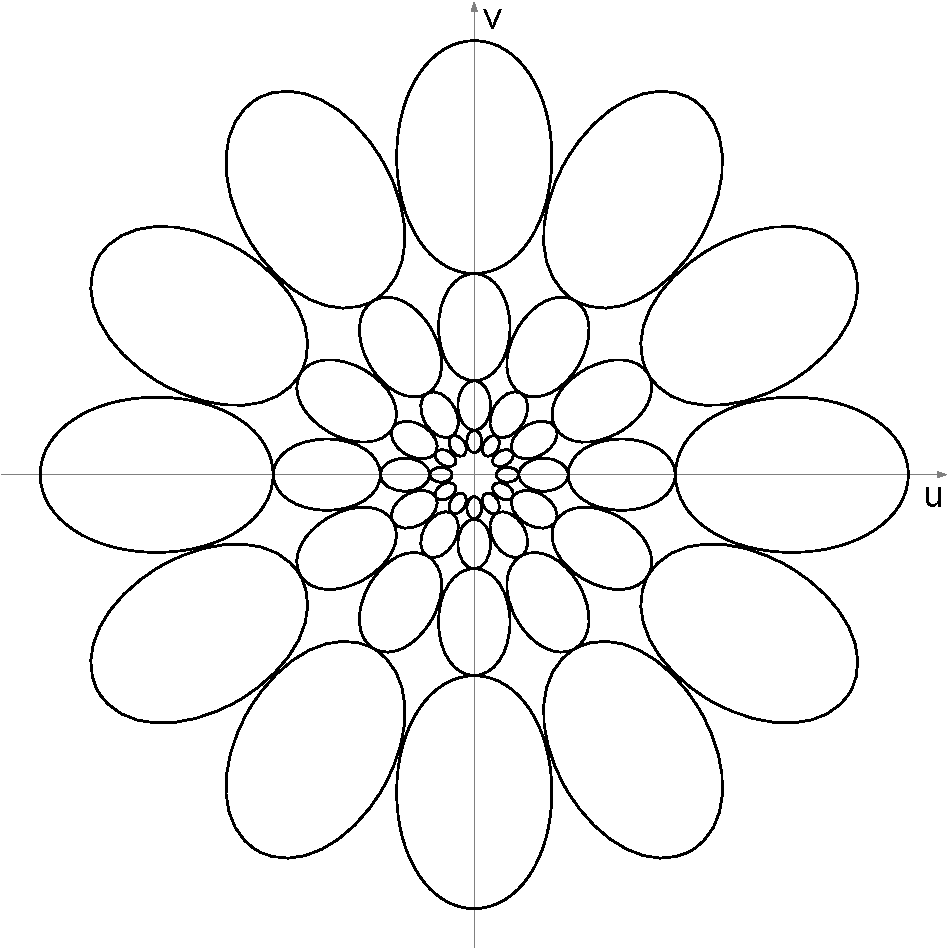
\includegraphics[width=0.5\textwidth]{gabor_tiling_cropped}
    \caption[Tiling of Gabor wavelets]{
        Tiling of Gabor wavelets. Note that due to the elliptical shape of the
        wavelets, some parts of the spectrum are left uncovered. (Image
        inspired by Manjunath and Ma \autocite{manjunath_texture_1996})
        }
    \label{fig:gabor_tiling}
\end{figure}

\subsection{The Continuous Curvelet Transform}\label{sec:background_cct}

The formulation of the continuous curvelet transform (CCT) by Candes and Donoho
\autocite{candes_curvelets:_2000} was based on Candes' previous definition and
expansion of the ridgelet transform \autocite{candes_ridgelets:_1998}. In that
publication they looked at the state of research into efficient representations
of edge discontinuities. They based their research on two realisations:
\begin{enumerate}
    \item A nonadaptive approach of signal approximation can compete with many
        of the adaptive schemes prevalent in previous research. At the same
        time the non-adaptivity comes with a greatly reduced computational
        overhead and reduced requirements for a priori knowledge. Obtaining
        that knowledge in the presence of blurred or noisy data can sometimes
        be unfeasable.
    \item Wavelet transforms can represent point singularities in a signal of
        up to two dimensions in a near-ideal manner, but fail to perform
        equally well on edges: Given a two-dimensional object in signal $f$, that
        is smooth except for discontinuities along a curve, a wavelet
        approximation $\tilde{f}^W_m$ from the $m$ largest coefficients
        exhibits an error of
        \begin{equation*}
            \| f - \tilde{f}^W_m \|^2 \propto m^{-1} \text{, for } m \rightarrow \infty
        \end{equation*}
        since up to $O(2^j)$ localized wavelets are needed to represent the
        signal along the edge. That falls short of what an approximation
        $\tilde{f}^T_m$ using a series of $m$ adapted triangles could achieve:
        \begin{equation*}
            \| f - \tilde{f}^T_m \|^2 \propto m^{-2} \text{, for } m \rightarrow \infty
        \end{equation*}
\end{enumerate}

They showed that a similarly precise approximation can be achieved by combining
Candes' ridgelet analysis \autocite{candes_ridgelets:_1998} with smart
windowing functions and bandpass filters. The steps of the transformation were
described as follows:

\begin{enumerate}
    \item Decomposition of the signal into subbands of scale-dependent size
    \item Partitioning of each subband into squares
    \item Normalisation of each square to unit scale
    \item Analysis of each square in an orthonormal ridgelet system
\end{enumerate}

The result was the formulation of a decomposition that matched the parabolic
scaling law $width \propto length^2$ often observed in curves.

The above formulation became known as the curvelet 99 transform when Candes and
Donoho revised it soon after \autocite{candes_new_2004}. The new version is not
dependent on ridgelets and aims to remove some shortcomings of the curvelet 99
transform, namely a simpler mathematical analysis, fewer parameters and
improved efficiency regarding digital implementations, which will be described
later.

The curvelet transform in $\mathbb{R}^2$ works by localising the curvelet
waveforms in the time domain. The "mother" curvelet waveform $\varphi_j(x)$ is
defined using two frequency domain windows $W(r)$, the "radial window" (Figure
\ref{fig:curvelet_frequency_windows_radial}), and $V(t)$, the "angular window"
(Figure \ref{fig:curvelet_frequency_windows_angular}). These windows must obey
the admissibility condition for wavelets. They can be combined in $U_j$ (Figure
\ref{fig:curvelet_frequency_windows_combined}):
\begin{equation*}
    U_j(r, \theta) = 2^\frac{-3j}{4} W(2^{-j}r) V(\frac{2^{\lfloor\frac{j}{2}\rfloor}\theta}{2 \pi}).
\end{equation*}

\begin{figure}[h]
    \centering
    \subfloat[Radial window]{%
        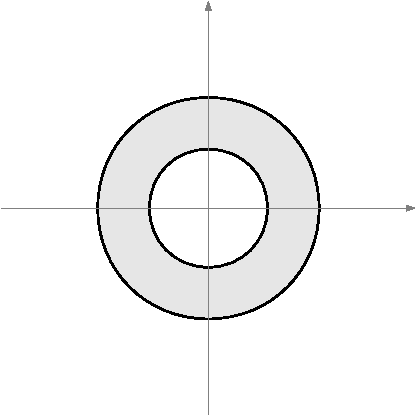
\includegraphics[width=0.45\textwidth]{curvelet_frequency_windows_radial_cropped}%
        \label{fig:curvelet_frequency_windows_radial}%
    }
    \quad
    \subfloat[Angular window]{%
        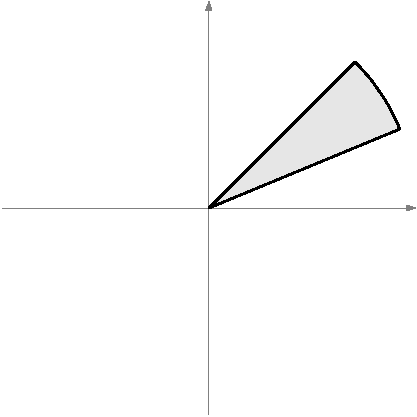
\includegraphics[width=0.45\textwidth]{curvelet_frequency_windows_angular_cropped}%
        \label{fig:curvelet_frequency_windows_angular}%
    }
    \quad
    \subfloat[Combined window]{%
        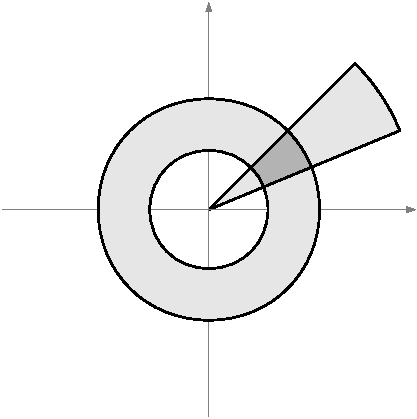
\includegraphics[width=0.45\textwidth]{curvelet_frequency_windows_combined_cropped}%
        \label{fig:curvelet_frequency_windows_combined}%
    }
    \quad
    \subfloat[Complete coronisation]{%
        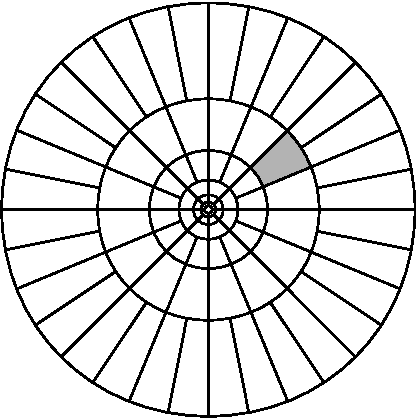
\includegraphics[width=0.45\textwidth]{curvelet_frequency_windows_corona_cropped}%
        \label{fig:curvelet_frequency_windows_corona}%
    }
    \caption[Curvelet frequency windows]{
        The window $W(2^{-j}r)$ at scale $2^j$
        \subref{fig:curvelet_frequency_windows_radial} is combined with the
        window $V(t)$ \subref{fig:curvelet_frequency_windows_angular} to form a
        support wedge for the curvelet
        \subref{fig:curvelet_frequency_windows_combined}. The wedge roughly
        obeys a $width \propto length^2$ relation.
        \subref{fig:curvelet_frequency_windows_corona} shows the wedge within a
        schema of the complete tiling in frequency domain.
    }
    \label{fig:curvelet_frequency_windows}
\end{figure}

The waveform $\varphi_j$ can then be expressed as being the inverse Fourier
transform of $\hat{\varphi}_j = U_j$ and all curvelets of a scale $2^{-j}$ can
be derived by
\begin{itemize}
    \item rotating $\varphi_j$ by a sequence of equispaced rotation angles
        $\theta_l = 2 \pi \cdot 2^{-\lfloor\frac{j}{2}\rfloor} \cdot l$ with $l
        = 0,1,\dots$ such that $0 < \theta_l < 2 \pi$ and
    \item translating $\varphi_j$ by a sequence of offsets $k = (k_1, k_2) \in \mathbb{Z}^2$:
\end{itemize}
\begin{equation} \label{eq:continuous_curvelet}
    \varphi_{j,k,l}(x) = \varphi_j(R_{\theta_l}(x - x_k^{(j,l)})),
\end{equation}
where $x = (x_1, x_2)$, $R_{\theta}$ is the rotation matrix for angle $\theta$
and $x_k^{(j,l)} = R_{\theta_l}^{-1}(k_1 \cdot 2^{-j}, k_2 \cdot
2^{-\frac{j}{2}})$.

\begin{figure}[h]
    \centering
    \subfloat[Coarse Curvelet waveform in time and frequency domain]{%
        \plotgraphics{curvelet_examples/curvelet_1_time.png}{194}{320}{194}{320}{$x_1$}{$x_2$}%
        \plotgraphics{curvelet_examples/curvelet_1_frequency.png}{0}{512}{0}{512}{$\omega_1$}{$\omega_2$}%
        \label{fig:curvelet_example_1}
    }
    \quad
    \subfloat[Fine Curvelet waveform in time and frequency domain]{%
        \plotgraphics{curvelet_examples/curvelet_2_time.png}{194}{320}{194}{320}{$x_1$}{$x_2$}%
        \plotgraphics{curvelet_examples/curvelet_2_frequency.png}{0}{512}{0}{512}{$\omega_1$}{$\omega_2$}%
        \label{fig:curvelet_example_2}
    }
    \caption[Curvelet waveforms in time and frequency domain]{
        Curvelet waveforms on coarse \subref{fig:curvelet_example_1} or fine
        \subref{fig:curvelet_example_2} scale with time domain shown on the
        left and frequency domain shown on the right side.
    }
    \label{fig:curvelet_examples}
\end{figure}


Each curvelet coefficient $c(j, l, k)$ can then be calculated as the inner
product of $f \in L^2(\mathbb{R}^2)$ and curvelet $\varphi_{j, l, k}$:
\begin{equation} \label{eq:continuous_curvelet_coefficient}
    c(j, l, k) := \langle f, \varphi_{j, l, k} \rangle = \int_{\mathbb{R}^2} f(x) \overline{\varphi_{j, l, k}(x)} dx
\end{equation}

As visible in figure \ref{fig:curvelet_frequency_windows_corona} curvelets also
have non-directional components at the coarsest scale, similar to those found
in the wavelet transform. Those curvelets will be defined using a special
low-pass filter window $W_0$, which is characterized as being the remainder of
the tiling not covered by the previously described radial windows:
\begin{equation*}
    |W_0(r)^2| + \sum_{j \geq 0} |W(2^{-j}r)|^2 = 1
\end{equation*}
With the help of window, defining the coarse scale curvelet $\varphi_{j_0, k}$
via its Fourier transform is straightforward:
\begin{equation} \label{eq:continuous_coarse_curvelet}
    \varphi_{j_0, k}(x) = \varphi_{j_0}(x-2^{-j_0}k), \hat{\varphi}_{j_0}(\omega) = 2^{-j_0}W_0(2^{-j_0}|\omega|),
\end{equation}
where $k = (k_1, k_2) \in \mathbb{Z}^2$.

Note that, in contrast to the Gabor wavelets (Figure \ref{fig:gabor_tiling}),
there is no gap in the curvelet tiling, so no information is lost.

\subsection{The Fast Discrete Curvelet Transform}\label{sec:background_fdct}

Based on the above definition of the continuous curvelet transform, a team
around the authors of the original curvelet publication presented two digital,
discrete implementations of the transform: the Fast Discrete Curvelet Transform
(FDCT) \autocite{candes_fast_2006}. The implementations have been described in
2D and 3D, but since this paper deals exclusively with 2D images, the
explanation below will also be restricted to two dimensions.

The digital versions of the transforms operate on arrays $f[t_1, t_2]$ with $0
\leq t_1, t_2 < n$ to produce coefficients $c^D(j, l, k)$ in a way
consistent with the continuous version (Equation
\ref{eq:continuous_curvelet_coefficient}):
\begin{equation}
    c^D(j, l, k) := \sum_{0 \leq t_1, t_2 < n} f[t_1, t_2] \overline{\varphi_{j, l, k}^D[t_1, t_2]}.
\end{equation}

Since the windows used in the continuous form are based on rotations and dyadic
coronae, they are not well suited for use with cartesian arrays. The discrete
formulation substitutes them with appropriate concepts. Instead of concentric
annuli, the window function $W^D_j$ generates concentric, square "rings" using
the square windows $\Phi_j(\omega_1, \omega_2) = \phi(2^{-j}\omega_1)
\phi(2^{-j}\omega_2)$, with $\phi$ being a low-pass 1D window:
\begin{equation*}
    W_j^D(\omega) = \sqrt{\Phi_{j+1}^2(\omega) - \Phi_j^2(\omega)}, \quad j \geq 0.
\end{equation*}
The rotation matrix $R_{\theta}$ is replaced by the shear matrix $S_{\theta}$
to create the combined window function
\begin{equation*}
    U_{j, l}^D := W_j^D(\omega) V_j(S_{\theta_l}\omega).
\end{equation*}
The sequence $\theta_l$ is defined as a sequence of equispaced slopes
$\tan(\theta_l) := l \cdot 2^{- \lfloor \frac{j}{2} \rfloor}$ with
$l=-2^{\lfloor \frac{j}{2} \rfloor}, \dots, 2^{\lfloor \frac{j}{2} \rfloor} -
1$.

Special attention must be paid to creating the windows, that touch the
diagonals, to ensure
\begin{equation*}
    \sum_{j} \sum_{l} | U_{j, l}^D (\omega)|^2 = 1
\end{equation*}
holds, so the tiling obeys the admissibility condition just like in the
continuous case. Figure \ref{fig:curvelet_frequency_windows_discrete} shows a
tiling of all $U_{j, l}^D$.

\begin{figure}[h]
    \centering
        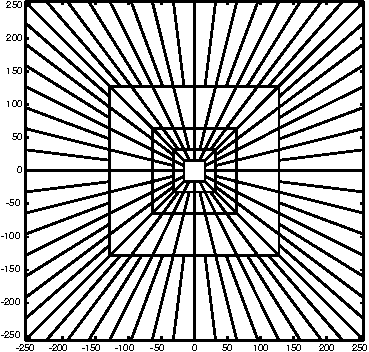
\includegraphics[width=0.5\textwidth]{curvelet_frequency_windows_discrete_cropped}
    \caption[Discrete frequency tiling using concentric squares]{
        Discrete frequency tiling using concentric squares (from Candes et al.\
        \autocite{candes_fast_2006})
    }
    \label{fig:curvelet_frequency_windows_discrete}
\end{figure}

\subsubsection{FDCT using unequispaced FFTs}

The first implementation of the discrete curvelet transform transfers the input
array $f[t_1, t_2]$, $0 \leq t_1, t_2 < n$ into the Fourier domain to obtain
$\hat{f}[n_1, n_2]$:
\begin{equation*}
    \hat{f}[n_1, n_2] = \sum_{t_1, t_2 = 0}^{n - 1} f[t_1, t_2] e^{- \frac{i 2 \pi (n_1 t_1 + n_2 t_2)}{n}}, \quad -\frac{n}{2} \leq n_1, n_2 < \frac{n}{2}
\end{equation*}

The obtained Fourier samples need to be interpolated for each pair of scale $j$
and angle $l$ to match the grid of the sheared support window $U_j^D[n_1, n_2]$
. The authors achieve this by resampling $\hat{f}$ on the grid
implied by the sheared window for each angle via a series of 1D fast Fourier
transforms.  These transforms represent a polynomial interpolation of each
"column" of the parallelogram $P_j$ containing the sheared window (Figure
\ref{fig:curvelet_usfft_tiling}), that can be computed with a $O(n^2 \log n)$
complexity in a sufficiently exact approximation.

This yields an object $\hat{f}[n_1, n_2 - n_1 \tan \theta_l]$ for $(n_1, n_2)
\in P_j$, that can be multiplied with the window $U_j^D$ described above in
order to create a localized "wedge" with the orientation $\theta_l$:
\begin{equation*}
    f_{j, l}^D[n_1, n_2] = \hat{f}[n_1, n_2 - n_1 \tan \theta_l] U_j^D[n_1, n_2]
\end{equation*}

The discrete curvelet coefficients $c^D(j, l, k)$ can then be calculated by
applying the inverse 2d Fourier transform:
\begin{equation*}
    c^D(j, k, l) = \sum_{n_1, n_2 \in P_j} \hat{f}[n_1, n_2 - n_1 \tan \theta_l] U_j^D[n_1, n_2] e^{i 2 \pi \left(\frac{k_1 n_1}{L_{1, j}} + \frac{k_2 n_2}{L_{2,j}}\right)},
\end{equation*}
in which $L_{1, j}$ and $L_{2, j}$ are the length and width of the rectangle supporting $U_j^D$.

\begin{figure}[h]
    \centering
    \subfloat[Sheared USFFT tiling]{%
        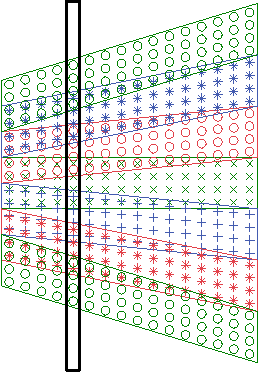
\includegraphics[width=0.35\textwidth]{curvelet_usfft_tiling_column_cropped}%
        \label{fig:curvelet_usfft_tiling}%
    }
    \quad
    \subfloat[Sheared tiling for wrapping]{%
        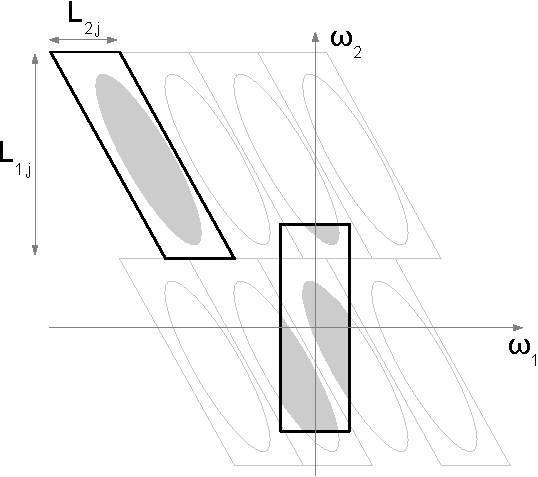
\includegraphics[width=0.55\textwidth]{curvelet_wrapping_cropped}%
        \label{fig:curvelet_wrapping_tiling}%
    }
    \caption[Frequency tilings for USFFT and wrapping]{
        \subref{fig:curvelet_usfft_tiling} illustrates the respective grid for
        each parallelogram containing several sheared support windows of the
        "east quadrant". The box highlights one of the columns, that represent
        one of the 1D polynomial interpolation problems solved for resampling.
        In \subref{fig:curvelet_wrapping_tiling}, the parallelogram $P_{j ,l}$
        is shown on top of the tilted tiling of a curvelet in frequency domain.
        Due to the periodicity, the rectangle in the center contains the same
        curvelet, but has a much smaller axis aligned bounding box for the FFT
        to operate on. Both images have been adapted from Candes et al.\ 
        \autocite{candes_fast_2006}.
    }
    \label{fig:curvelet_discrete_tilings}
\end{figure}

\subsubsection{FDCT using wrapping}

As before, FDCT using wrapping first calculates $\hat{f}[n_1, n_2]$ with
$-\frac{n}{2} \leq n_1, n_2 < \frac{n}{2}$ as the Fourier transform of the
input $f$. The sample is then localized by multiplying it with a window $U_{j,
l}^D$ for each angle $j$ and scale $l$:
\begin{equation*}
    d_{j, l}[n_1, n_2] = U_{j, l}^D \hat{f}[n_1, n_2]
\end{equation*}

To avoid the computationally costly interpolation step required in the USFFT
approach, this method keeps the rectangular grid of the input signal. Because
an axis-aligned bounding box of the window $U_j^D$ in Fourier domain cannot
maintain the $width \propto length^2$ proportions of the window, applying an
inverse Fourier transform on such a bounding box in general would lead to
significant oversampling of the coefficients and thereby increase the memory
requirements for fine scale curvelets beyond that of the the USFFT approach. In
order to circumvent that, the authors utilize the periodic nature of the
Fourier transform and propose generating a periodically wrapped version of the
fourier samples. For $P_{j, l}$ as the bounding parallelogram of $U_{j, l}^D$,
$L_{1, j}$ and $L_{2, j}$ are the period lengths by which to translate $P_{j,
l}$ in the horizontal and vertical direction to produce a suitable tiling for
each orientation $\theta_l$ (Figure \ref{fig:curvelet_discrete_tilings}). Thus,
the wrapped, localized data are
\begin{equation*}
    f_{j, l}^D[n_1, n_2] = W d_{j, l}[n_1, n_2] = \sum_{m_1 \in \mathbb{Z}} \sum_{m_2 \in \mathbb{Z}} d_{j, l}[n_1 + m_1 L_{1, j}, n_2 + m_2 L_{2, j}]
\end{equation*}
with $0 \leq n_1 < L_{1, j}$ and $0 \leq n_2 < L_{2, j}$, which gives a
rectangle of size $L_{1, j}$ times $L_{2, j}$.

Again, the discrete curvelet coefficients $c^D(j, l, k)$ can then be collected
using the inverse 2d Fourier transform:
\begin{equation*}
    c^D(j, k, l) = \sum_{n_1, n_2 \in P_j} f_{j, l}^D[n_1, n_2] e^{i 2 \pi \left(\frac{k_1 n_1}{L_{1, j}} + \frac{k_2 n_2}{L_{2,j}}\right)}.
\end{equation*}

\subsection{gPb Contour Detection}\label{sec:background_gpb}

Maire et al.\ \autocite{maire_using_2008} describe an improvement of the
contour detector published by Martin et al.\ \autocite{martin_learning_2004},
that includes global information in addition to local cues. The
orientation-specific local parameters $G_i$ extracted from a circular
neighborhood around the location $(x, y)$ are brightness, color and texture
gradients on three scales. They are summarized as a coefficient $mPb(x, y,
\theta)$ using a weighted sum with weights $\alpha_i$:
\begin{equation*}
    mPb(x, y, \theta) = \sum_{i=1}^9 \alpha_i G_i(x, y, \theta)
\end{equation*}

The global combonent $sPb(x, y, \theta)$ is the result of applying a
filterbank of directional gaussian derivatives to a set of $k$ generalized
eigenvectors $v_j$, $j \in 1, \dots, k$. The linear system these eigenvectors are
obtained from has an affinity matrix derived from the intervening contour cue
\autocite{fowlkes_learning_2003}. The linear combination of the individual
directional derivatives then represents the large-scale contours in the image:
\begin{equation*}
    sPb(x, y, \theta) = \sum_{j=1}^k \frac{1}{\sqrt{\lambda_j}} sPb_{v_j}(x, y, \theta)
\end{equation*}

A further linear combination of the local component $mPb$ and the global
component $sPb$ with learned weights $\alpha_i$ and $\gamma$ provides a
detailed map of contours in the image while limiting the amount of clutter
compared to a purely local contour detector:
\begin{equation*}
    gPb(x, y, \theta) = \sum_{i=1}^9 \alpha_i G_i(x, y, \theta) + \gamma \cdot sPb(x, y, \theta)
\end{equation*}

From these directional contour maps, Arbeláez et al.\ derived a hierarchical
contour detector \autocite{arbelaez_contours_2009}, that conditionally joins
adjacent regions to obtain closed-contour maps of high quality.



%OLD STUFF BELOW

%Most approaches can be characterized by looking at three stages in their processing pipeline:

%\begin{description}
    %\item[Input format] The structure of the input data determines the amount of information available to the subsequent processing steps. Possible preprocessing steps include color space conversion, scaling and edge extraction.
    %\item[Extracted features] Many algorithms produce a large number of coefficients that can be reduced to a set of feature coefficients using by techniques such as vector quantization or principal component analysis (PCA).
    %\item[Distance metric] In order to rank the images according to similarity a metric is used to calculate the distance in feature space between two sets of feature coefficients. The selection of a metric is often closely coupled with the feature extraction algorithm.
%\end{description}

%\subsection{input format}
%Complete vs incomplete sketches, intra-/cross-domain

%\subsection{features}

%\begin{itemize}
    %\item bag of features from k-means clustered visual words [video google]
    %\item histogram of oriented gradients [chalechale + refs]
%\end{itemize}

%\subsection{metric}

%\begin{itemize}
    %\item after ranking using euclidean distance, rank by spatial similarity [video google]
    %\item Earth Mover's distance? [rubnerljcv00]
%\end{itemize}
